\documentclass[acmsmall]{acmart}

\usepackage{multicol}
\AtBeginDocument{%
  \providecommand\BibTeX{{%
    \normalfont B\kern-0.5em{\scshape i\kern-0.25em b}\kern-0.8em\TeX}}}

%% These commands are for a JOURNAL article.
\acmJournal{JACM}
\acmVolume{1}
\acmNumber{1}
\acmArticle{1}
\acmMonth{3}


\def\RR{\,$\mathbb{R}$\,}
\def\QQ{\,$\mathbb{Q}$\,}
\def\ZZ{\,$\mathbb{Z}$\,}
\def\n{\,$\char`\\ n$\,}
\def\tab{\,$\quad \quad$\,}
\def\small{\,\par \smallskip\,}
\def\med{\,\par \medskip\,}
\def\big{\,\par \bigskip\,}
\newcommand{\csfont}[1]{\fontfamily{cmtt}\selectfont #1}

\begin{document}

%%
%% The "title" command has an optional parameter,
%% allowing the author to define a "short title" to be used in page headers.
\title{CSE 489 Final Report: Analogous CPU}

%%
%% The "author" command and its associated commands are used to define
%% the authors and their affiliations.
%% Of note is the shared affiliation of the first two authors, and the
%% "authornote" and "authornotemark" commands
%% used to denote shared contribution to the research.
\author{Matthew C. Lindeman}
\email{matthew.lindeman@student.nmt.edu}
\orcid{1234-5678-9012}
\affiliation{%
  \institution{New Mexico Institute of Mining and Technology}
  \streetaddress{801 Leroy Pl}
  \city{Socorro}
  \state{New Mexico}
  \country{USA}
  \postcode{87801}
}

%%
%% By default, the full list of authors will be used in the page
%% headers. Often, this list is too long, and will overlap
%% other information printed in the page headers. This command allows
%% the author to define a more concise list
%% of authors' names for this purpose.
\renewcommand{\shortauthors}{Matthew C. Lindeman}

%%
%% The abstract is a short summary of the work to be presented in the
%% article.
\begin{abstract}
  This project is meant to be an environment from which the user can test
  scheduling algorithms to duduce logical statements about them in a reasonable
  manner. A reasonable manner in this instance, is a way in which the only
  interface for the user to interact with is the implementation of the
  scheduling algorithm itself in native C code. In this manner, roughly, scheduling algorithms
  can be judged based off of performance with respect to a particular feature.
  For example, scheduling algorithm X may be better at handling IO processes in
  short bursts. This project is the collection of code that represents the base
  unit of execution, process list in a manner from which data can
  generically be piped in and out, and the data collection elements bassed of
  the base unit of execution. Additionally, as a proof of concept, I have
  implemented the lottery scheduling algorithm and used the system to collect
  data over it which I will present as an example of what the system can do with
  respect to analysis.
  \par
  {\it Please see the source code as it was intended to be veiwed by the developer
  (complete with automatic markdown reader) by accessing
  https://github.com/millipedes/Scheduling-Simulator with a modern non-text
  based browser.}
\end{abstract}


%% Keywords. The author(s) should pick words that accurately describe
%% the work being presented. Separate the keywords with commas.
\keywords{CPU, Operating System Scheduling, Process Scheduling}


%% This command processes the author and affiliation and title
%% information and builds the first part of the formatted document.
\maketitle

\begin{multicols}{2}
    \section{Overveiw of the Project}
    For a visual reference please see the uml document hosted under the
    source project directory {\csfont{documentation/plant/uml$\_$figure.png}}.
    \subsection{Fundemental Structure}
    For the system to be opaque to the user, a scheduling algorithm must be
    well defined. Thus we will define it using three variants: $\alpha$,
    $\beta$, and $\gamma$. Which are defined repspectively to be the following:
    \begin{enumerate}
      \item $\alpha$ - the hardware environment which the algorithm runs on
        (alogous to the base unit of execution in the project as work is
        measured as a scalar not a vector).
      \item $\beta$ - The characteristics that the scheduling algorithm
        associates with each process (this can be the empty set and in the code
        is analogous to the process and process$\_$list data objects). The
        architecture of this project allows for dynamic $\beta$. The way that
        this was implemented was using the relationship between process and
        proc$\_$list. Each of these structures have generic ports to custom data
        types. This is where work quantity being a scalar not a vector becomes
        useful as regarless of the data types required by the algorithm, the end
        quantity of work being performed (what is recorded by each process) can
        be ported to this scalar work quantity which is universal.
      \item $\gamma$ - The scheduling algorithm itself (this is the primarily
        interesting variant, however to show the functionality of the system I
        have implemented an instance of the lottery scheduling algorithm with
        the project infrastructure).
    \end{enumerate}
    Using these variants it becomes clear that a system capable of handling a
    varrying $\alpha$, $\beta$, and $\gamma$ in extensible C code must have
    the following:
    \begin{itemize}
      \item Have a process tracking infrastructure capable of communitcating
        with a generic interface, both storing and writing data.
      \item The units of the process tracking system must be capable of having
        varrying attributes.
      \item A generic and universal way of representing work.
    \end{itemize}
    The uml diagram contains a full accounting of the project, but some of the
    more fundemental and high level objects can be used to explain the
    functionality of the system.
    \par
    Some of the  genericity of the following subsystems have yet to be
    implemented in the project, as currently the lottery scheduling algorithm
    has been hard coded with respect to types in the source code.  These can be replaced by void
    pointers instead to achieve this genericity and the code functions in the
    same manner.
    \par
    \textbf{cpu$\_$t} - This is the interface with the direct work of the system
    (i.e. how many and or to what degree have processes been completed for a
    given time quantum). The genericity is achieved here by having a generic
    unit of execution. I.e. at runtime it can be assigned to be an ARM
    architecture processor, x86 architecture processor, etc. as its attribute of
    execution is user defined.
    \par
    \textbf{process} - This structure in the code can handle the data provided
    by the scheduling algorithm in a manner suitable for the particular
    algorithm. See later in the paper for this explained for lottery scheduling.
    \par
    \textbf{proc$\_$list} - This structure contains a generic way to
    interact with the scheduling algorithm's data structures.
    \par
    \textbf{lottery/base} - The particular $\gamma$ which was implemented for
    the project as a proof of concept.
    \par
    \textbf{base} - In the description of the implementation of the lottery
    scheduling algorithm, the researchers who wrote the paper mentioned a
    particular data structure which was used to more efficiently track tickets.
    This structre involded having pointers from the threads to the currently
    executing process's tickets which in turn had pointers to processes with
    pointers to tickets and this process is repeated until the process is
    pointing the the base structure of currency.
    \par

\section{List of Supported variants}
  The following are the vartiants that can be changed that would be of use to
  the user. Additionally, the structural extensibility of the project is
  discussed. Any all-caps reference is a definition under the source project
  file: {\csfont{src/constants$\_$macros/include/constants.h}}.
  \subsection{$\alpha$}
    Structural Extensibility:
    \begin{itemize}
      \item The pointer between cpu$\_$t and what is currently thread can be
        modified to change the way in which tasks are handled (i.e. a cpu could
        point to another cpu changing the way it executes the scheduling
        algorithm).
    \end{itemize}
    Data Variants:
    \begin{itemize}
      \item The number of threads that the given CPU is utilizing.
        (THREAD$\_$NO).
      \item The scalar quantity of work that each thread is executing per time
        quantum (THREAD$\_$WORK).
    \end{itemize}
  \subsection{$\beta$}
    Structural Extensibility:
    \begin{enumerate}
      \item There exists a pointer from proc$\_$list to process which allows for
        the downward flow of data.
      \item proc$\_$list and process both void pointer data ports to recieve
        data from a scheduling algorithm.
    \end{enumerate}
    Data Variants:
    \begin{enumerate}
      \item The total number of processes that the process list can have
        (P$\_$LIST$\_$INITIAL$\_$SIZE).
      \item The total proportion of I/O processes to memory related processes
        (MEM$\_$PROP).
      \item The maximum number of processes generated by the system for each
        time quantum. It is the maximum as all process quantity generation is
        random (MAX$\_$NG$\_$PROCS).
      \item The maximum quantity of work that a process requires to be
        completed. Again, is the maximum as all process work quantity generation
        is random (MAX$\_$PROC$\_$WORK).
    \end{enumerate}
  \subsection{$\gamma$}
    Structural Extensibility:
    \begin{itemize}
      \item The algorithm implementation can be changed dynamically under the
        condition it feeds data into the proper ports with the surounding
        system.
      \item The algorithm data structures can be changed dynamically under the
        condition that it feeds data into the proper ports of the surounding
        system.
    \end{itemize}
    Due to the nature of $\beta$ there should exist no variance in the data
    related to $\gamma$.

\section{Lottery Scheduling System}
  As previously mentioned, as a proof of concept of the system itselt I
  implemented the lottery scheduling alghorithm as a sample $\gamma$ (note that
  the uml diagram is relflective of this). Below I will describe the manner in
  which $\alpha$, $\beta$, and $\gamma$ were realized in the system.
  \subsection{$\alpha$ Implementation}
    This is done via CPU with threads that have direct work quantity that they
    fulfil each time quantum.
  \subsection{$\beta$ Implementation}
    This is where this project best illustrates how it is extensible. In order
    to discuss why, first we must reveiw the way in which the lottery scheduling
    algorithm determines where its currencies are backed from.
    \par
    The way in which this was implemetned for the lottery scheduling algorithm
    was by using a base currency structure which interfaces with proc$\_$list
    via pointers and ticket$\_$bundles which interact with process replicating
    (with a few extra explicit edges in the representative graph of the data
    structure) the process described in the lottery scheduling algorithm paper.
  \subsection{$\gamma$ Implementation}
    The entirety of the lotttery scheduling interface itself can be found in
    Appendix figure 1. The process list can be used to alter and get data, but
    under the hood it is the user defined base and ticket$\_$bundle structures
    that fundementally store the data.

\section{Example Experiment Using the Subsystem}
  \subsection{Premise}
    Suppose a user wanted to know the approximate threshold at which the
    quantity of processes will either be completed per each time quantum by the
    processor and the threshold at which the number of processes tends towards
    infinity. From the system documentation we can see that there are several
    relevant parameters, but this particular user is interested only in the
    process's data impacts on these thresholds.  This narrows it down to two
    vartiants:
    \begin{itemize}
      \item Process Data Variant - MAX$\_$NG$\_$PROCS (the max number of
        processes that can be generated given a particular time quantum).
      \item Process Data Variant - MAX$\_$PROC$\_$WORK (the maximum amount of
        work that it will require to complete a generated process).
    \end{itemize}
    Now that the variants are decided upon, the user will chose which aspect(s)
    of the system the wish to examine in relationship to these variants. For
    this example, we will observe the affect of these variants on the
    proc$\_$list across time quantums.
    \par
    As it would be standard to do (and this project makes trivial) we must state
    our assumptions:
    \begin{enumerate}
      \item Local system (i.e. single CPU)
      \item 8 Threads
      \item 2000 Max process list size
      \item Threads Perform 30 Work per Time Quantum
    \end{enumerate}
    Let us conduct the following experiments with the above assumptions:
    \par
    \begin{tabular}{|c|ccccc|}
      \hline
      Test $\#$         & 1  & 2  & 3  & 4  & 5 \\
      \hline
      Max New Gen Procs & 5  & 5  & 5  & 10 & 15 \\
      \hline
      Max New Proc Work & 50 & 60 & 75 & 75 & 75 \\
      \hline
    \end{tabular}
    \par
    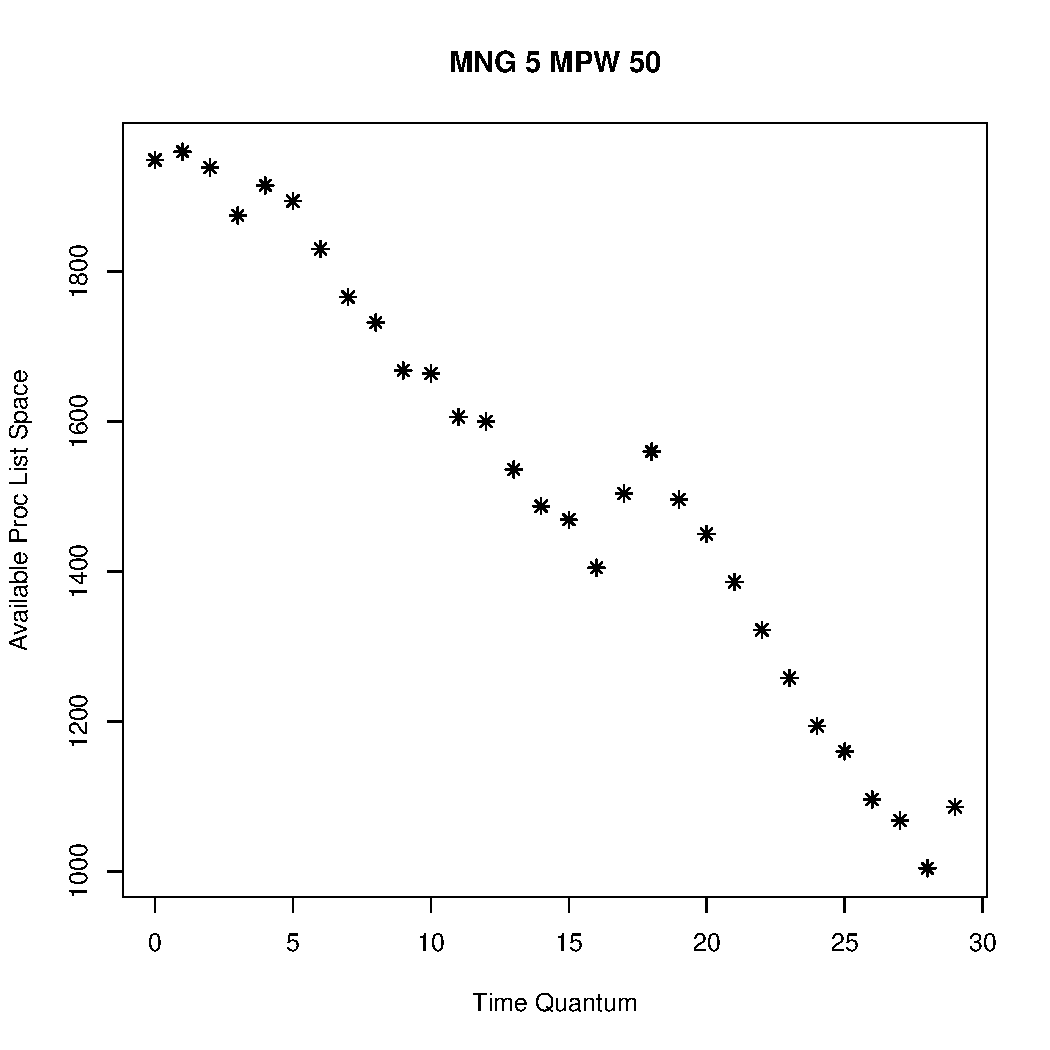
\includegraphics[scale=0.4, page=1]{{./firgures/data/Rplots.pdf}}
    \par
    This is the first test for which processes are introduced with low maximum
    potential work to be completed, and low maximum number of processes
    generated each generation. The user can see that this is unsustainable over
    time and that the available space will tend to 0.
    \par
    \includegraphics[scale=0.4, page=2]{{./firgures/data/Rplots.pdf}}
    \par
    This is the second test for which processes are introduced with slightly
    higher number of processes being generated each time quantum. The user
    can see that this is unsustainable over time and that the available space
    will tend to 0 even faster then when the potential work was lower.
    \par
    \includegraphics[scale=0.4, page=3]{{./firgures/data/Rplots.pdf}}
    \par
    This is the third test for which processes are introduced with higher new
    generation process generation. The user can see that this is
    unsustainable over time and that the available space will tend to 0 even
    faster then when the potential work was lower.
    \par
    Please note that available space becoming negative was a design oversight,
    as programmed, negative process list space is indicative of processes
    happening faster than the CPU can process them.
    \par
    \includegraphics[scale=0.4, page=4]{{./firgures/data/Rplots.pdf}}
    \par
    The fourth test. We can see that with a high number of process being
    generated each time quantum and a high potential work to complete each
    process that the CPU will be overwhelmed quickly.
    \par
    \includegraphics[scale=0.4, page=5]{{./firgures/data/Rplots.pdf}}
    \par
    The fifth test. Similarly to the fourth can see that with a high number of process being
    generated each time quantum and a high potential work to complete each
    process that the CPU will be overwhelmed even quicker.

\section{Conclusion}
  The results from the test experiment seem reasonable. Additionally, the
  interface between $\gamma$ and the system is just a matter of coding the
  implementation of the scheduling algorithm and its respective data sctructures
  in C then modifying conduct$\_$test(). For these reasons, I would argue that
  this tool accomplishes, at least at a base level, its goal.

\section{Project Next Steps}
  The next step would be 100$\%$ implementing the genericity to the clients that
  handle the work execution (i.e. tweaking the way that the cpu interacts with
  the scheduling algorithm).
  \par
  Additionally, implementing other algorithms to give some comparison among
  $\gamma$ would be a high priority for this project in the future.

\section{Final Scope of Project}
  \begin{itemize}
    \item 1350 lines of C code
  \end{itemize}

\end{multicols}
\section{References}
\begin{enumerate}
  \item Waldspurger, Weihl, Lottery Schedduling: Flexiblle Proportional-Share
    Management
  \item Moring, Schultz, Uetz, Approximation of stochastic scheduling: the
    power of LP-based piority policies.
  \item Scharbrodt, Schickingera, Steger, A new average analysis for completion
    time scheduling.
  \item Rothkopf, Scheduling with random service times.
  \item Weiss, Approximation results in parallel machines stochastic scheduling
  \item Megow, Uetz, Vredeveld, Models for stochastic online scheduling.
  \item Skutella, Uetz, stochastic Machine Scheduling with precedence
    constraints.
  \item Chandy, Renolds, Scheduling partially ordered tasts with posibilistic
    execution times.
  \item Graham, Lawler, Lenstra, Kan, Optimization and approximation in
    deterministic sequencing and scheduling: a servey
  \item Allahverdi, Gupta, Aldowaisan, A reveiw of scheduling reasearch
    involving setup consideration.
\end{enumerate}

\section{Appendix}
\begin{tabular}{c|l}
  \hline
  1 & void host$\_$lottery(thread * t, proc$\_$list * pl) $\{$ \\
  \hline
  2 & \tab time$\_$t ti; \\
  3 & \tab srand((unsigned) time($\&$ti)); \\
  4 & \tab int windex = (pl$->$b$->$total$\_$space - pl$->$b$->$available$\_$space); \\
  5 & \tab int winner = 0; \\
  6 & \tab if(windex > 0) $\{$ \\
  7 & \tab \tab winner = rand() $\%$ windex; \\
  8 & \tab $\}$ \\
  9 & \tab int reduction$\_$index = find$\_$ticket$\_$partition$\_$process$\_$index(pl, winner); \\
  10 & \tab if(pl$->$b$->$bid$->$size $>$ 0 $\&\&$ pl$->$p$\_$list$[$reduction$\_$index$]->$tb) $\{$ \\
  11 & \tab \tab reduce$\_$bundle(pl, t$->$work$\_$qty, pl$->$p$\_$list[reduction$\_$index]$->$tb$->$id); \\
  12 & \tab $\}$ \\
  13 & $\}$ \\
  \hline
\end{tabular}
\par
\small{Figure 1}


\end{document}
\endinput
